%
% T�TULO DEL CAP�TULO
%
\chapter{Planning and methodology
	\label{chapter_2}
}

This chapter explains what software development method was used in the project. We are strong believers in agile software development, above all for research oriented projects like this. In the next sections, some basic concepts of this development philosophy are introduced, as well as how it was applied in our project. Furthermore, a Gantt chart with the different steps and periods of the development is presented so that the reader can see how long each element of the project took. Since this is a project that requires a lot of research, it is difficult to plan ahead; because we do not know how long we are going to spend on a certain element. Finally we will give a cost table with the estimated project cost.

\section[Agile software development]{Agile software development}

Agile software development \cite{agiledev} is a combination of development methods that use iterative and incremental development, where requirements and solutions mature through collaboration between self-organizing, cross-functional teams. The motto of this method is ``embrace change''; that is why it encourages adaptive planning, evolutionary development and delivery, a time-boxed iterative approach, and promotes quick and flexible response to change.

\subsection[Agile manifesto]{Agile manifesto}

In February of 2001, several developers met at Snowbird, Utah resort, to debate different lightweight development methods. They published the \emph{Manifesto for Agile Software Development} \cite{agilemani} to define the approach that is now called agile software development. 

The conclusions that we can reach from the manifesto's items are described below:

\begin{itemize}
\item \textbf{Individuals and Interactions}: In agile development self-organization and motivation are really important. Other values promoted by the manifesto are co-location\footnote{The act of placing multiple individuals within a single location.} and pair programming\footnote{Two programmers work together at one workstation.}.
\item \textbf{Working software}: Working software will be utilized for more purposes than presenting documents to the client.
\item \textbf{Customer collaboration}: The software requirements cannot be fully realized from the beginning of the software development cycle, so being in touch with the customer is really important.
\item \textbf{Responding to change}: Agile development is keen on fast responses to change and continuous development.  
\end{itemize}

More principles are mentioned in the manifesto, some of them are:

\begin{itemize}
\item Customer satisfaction by rapid delivery of useful software.
\item Welcome changes even late in the development.
\item Working software is the principal measure of progress.
\item Maintaining a constant pace.
\item Cooperation between business people and developers. 
\item Build projects around motivated individuals.
\item Attention to technical excellence.
\item Simplicity.
\end{itemize}

Agile methods break down task into small increments with minimal planning and normally long-term planning is not directly involved. \emph{Iterations} are short timeframes that typically last from one to four weeks. A team works in each iteration through a full software development cycle; including planning, requirements analysis, design, coding, etc. This minimizes risk and facilitates adaptation to change. An iteration may not add enough new functionalities to warrant a market release, but the objective is to have an available release at the end of each iteration. 

Team composition does not depend on corporate hierarchies or corporate roles of team members. They normally have the responsability of completing tasks that deliver the required functionalities that an iteration requires. How to meet an iteration's objectives is decided individually.

The ``weight'' of the method depends on the type of project, the planning and order of tasks in a generalist project should not be the same as in a research project.  

Agile methods encourage face-to-face communication instead of written documents if possible. Most teams work in an open office (the \emph{bullpen}), which makes this type of communication easier. 

Each agile team contains a customer representative, that ensures that customer needs and company goals are aligned. 

Most agile methods encourage a routine that includes daily face-to-face communication among team members. In a brief session team members tell each other what they achieved the previous day, what they are going to do today and the problems that have appeared. 

As agile development emphasizes on working software as the primary measure of progress and has a clear preference in face-to-face communication this results in less written documentation than other methods. This does not mean that documentation should be disregarded, but that less emphasis is made on documentation because is not needed as much.

\subsection[XP]{Extreme programming}

Extreme Programming Explained \cite{XP} describes this method as a software-development discipline that lays out how to organize people to produce higher-quality software more productively.

XP tries to reduce the cost of requirement volatility by using short development cycles, rather than a really long one. In this teaching, change is inherent, inescapable and a desirable aspect of development projects, should be welcome with open arms and planned for in advance, instead to trying to cling to certain fixed requirements.  

Extreme programming also introduces a number of basic values, principles and practices on top of the agile programming principles.

\begin{itemize}
\item \textbf{Values}
	\begin{itemize}
		\item \textit{Communication:} To build a software system it is required to communicate the requirements to the developers. This is achieved through documentation.
		\item \textit{Simplicity:} It is encouraged to start simple and add extra functionality at a later time. The main difference between this method and others is focusing on design and coding that satisfies the needs of today and not tomorrow.
		\item \textit{Feedback:} From the system, customer and team. This is closely related to communication and simplicity.
		\item \textit{Courage:} Simplicity, refactoring and getting rid of code when necessary require courage.
		\item \textit{Respect:} Respect for others and yourself. Always think of the team when making changes and respect the work of everybody.
	\end{itemize}
	\item \textbf{Principles}
	\begin{itemize}
		\item \textit{Feedback:} This principle is most useful when is done frequently and promptly. Minimal delay between actions and feedback is key to learning and making changes.
		\item \textit{Assuming simplicity:} The fact of treating every problem as if its solution were really ``simple''. This doctrine stresses that big changes all at once do not work.
		\item \textit{Embracing change:} Change should be embraced instead of trying to work against it or avoid it.
	\end{itemize}
	\item \textbf{Practices}
	\begin{itemize}
		\item \textit{Informative workspace:} Build your workspace around your work. Anyone that visits your workspace should have a general idea of how the project is going in 15 minutes.  
		\item \textit{Sustainable pace:} Work as many hours as you can be productive. Overworking today and wasting the next two days is not good.
		\item \textit{User stories:} Plan using units of work that the client will understand. Having the stories on display will help with having an informative workplace and keeping track of progress. 
		\item \textit{Incremental design:} Invest in system design every day. Try to excel in designing the system so that it meets the day to day requirements.
		\item \textit{Pair programming:} A technique in which two programmers work together in a single workstation. 
		\item \textit{Continuous integration:} This technique helps to prevent integration problems. It consists on merging all developer working copies with a shared stable version of the software. 
		\item \textit{Ten minute build:} Build the complete system automatically and execute every test in 10 minutes. 
		\item \textit{Test-driven development:} Write automatic tests that fail before changing any code.
		\item \textit{Whole team:} Not only the developers should communicate between each other, the customer should also be available for questions.
		\item \textit{Sit together:} Have an open space available for the team. If it is not possible, video-conferences should be used to have more face to face time.
		\item \textit{Weekly cycle:} Start the week writing automated tests and then during the week implement them. 
		\item \textit{Quarterly cycle:} Plan for releases that will cover themes. Themes are broken down into stories for weekly cycles.  
	\end{itemize}
\end{itemize}

\subsection[Application]{Application}

We have used in our project several of the premises of agile software development. We have used approximately weekly or biweekly iterations focused on completing simple objectives that would yield working software. The work in each iteration has been constant and diligent, focusing always on completing the task at hand, but not avoiding changes if it was deemed necessary. 

Also several XP practices were used in the project. Such as user stories (see \figurename~\ref{story_cards}), were each planned functionality was broken up in stories if big enough. Then the effort to implement each story was estimated directly since the estimation units are simple enough to provide a rough estimate, but because of the nature of the project this estimates were not very precise even when estimating just small units. They were just meant as guidance and mainly used to keep track of progress.  Another practice followed was an informative workspace, the story cards were stuck to the wall so they were easily visible to everybody. They were also organized in groups, so the progress in each functional area was easily tracked.

\begin{figure}[h]
	\centering
	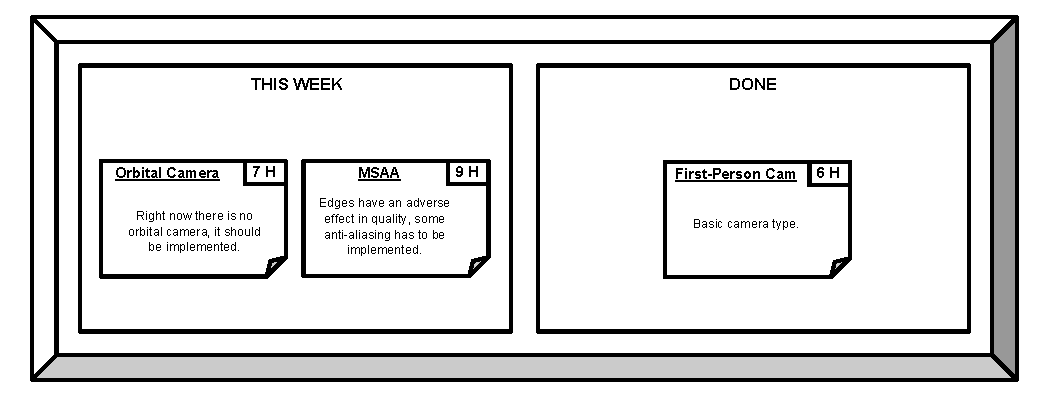
\includegraphics[scale=0.6]{figures/story_cards.pdf}
	\caption[Story cards]{
		In this image we can see a sketch of the structure of a story card and how they were organized.
	}
	\label{story_cards}
\end{figure}

Incremental design was also used, every day the design was reviewed and adapted to the new requirements. Lastly, a sustainable pace was kept. Because designing and implementing software is a creative process that requires insight, developers have to be rested, ready and motivated. To make the most of the worked time, the premise of coding for two hours straight without checking e-mails or other distractions was used, along with other similar productivity tricks. 

The meetings with my two advisors were kept on face-to-face basis when possible. In each meeting we would comment what had been achieved since the last one, laid out what the objectives were for the next iteration and talked about the roadblocks found on the task at hand. Whenever communication in person was not possible, e-mails were exchanged regularly if tasks where completed or any other event arised. 

To keep the code accessible by everyone in the team, up to date and well organized \textbf{Git} \cite{gitrev} version control software was used. Git is free software used to manage source code and keep distributed revision control. Every Git working directory is a repository with complete history and revision tracking capabilities. In this project it was essential to have a system like this in place, because of the research nature of the project. Ideas needed to be tried without wasting time on keeping tabs on the added code, Git makes this really easy and not problematic thanks to history and revision tracking.

Since the project is divided in two sub-projects (PCM and ToView\footnote{The visualizer, the main focus of this project.}), it was also necessary to manage the separate repositories in some way. With this in mind, \textbf{Redmine} \cite{redmine} was chosen to achieve our goal. This is a free and open source web-based tool for project management and bug tracking. It has support for multiple projects, a Gantt chart, calendar, support for multiple users, several types of repositories, news, wiki, etc. 

As this project is meant to be open source, this tool will allow the coordination of the efforts of future developments well after the end of this project. We believe this project will be a good fit for the ``bazaar type'' of development that other successful open source software has used. In this model, the code is developed openly for everyone to see. This type of development also encourages the participation of the user in the development process.      

We have also estimated the cost of the project as we can see in Table~\ref{cost_table}. It only includes human resources and hardware costs because all the software used was free.

\begin{table}
\begin{center}
\begin{tabular}{lcccr}
\toprule
Resource & Units & Hours & Cost per hour & Total \\
\midrule
  Software &  &   &  & 0 \euro \\
  Computer & 1 &   &  & 1800 \euro \\
  Analyst-programmer & 1 & 950 & 16 \euro & 15200 \euro \\
  \midrule
  &&&&17000 \euro\\
\bottomrule
\end{tabular}
\end{center}
\caption[Cost estimate]{
		Table showing the estimated cost of the project.
}
\label{cost_table}
\end{table}

Although because of the research nature of the project it was not possible to estimate how much time we would spend in each iteration, we provide a Gantt chart that depicts how the project iterations were performed after the fact (see \figurename~\ref{gantt_chart}).

\begin{landscape}
	\begin{figure}
		\centering
		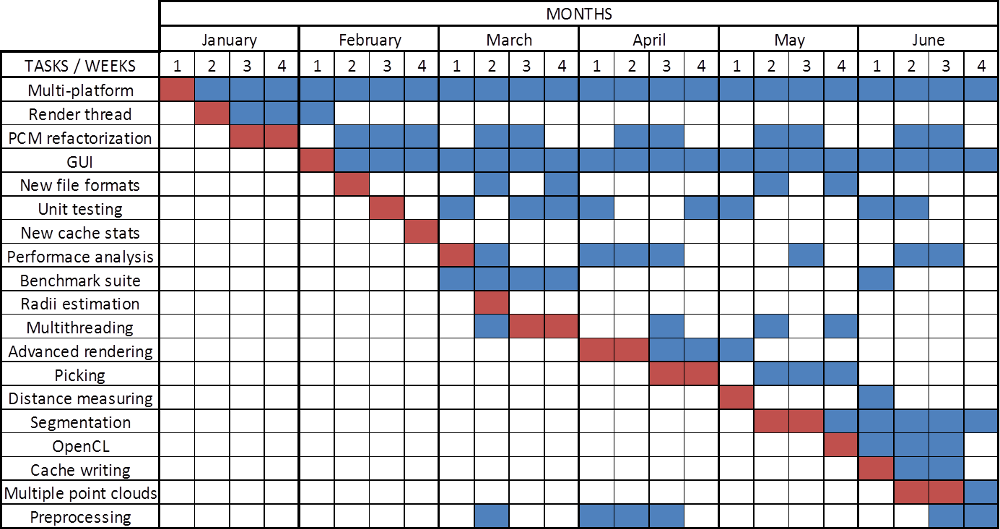
\includegraphics[scale=0.6]{figures/gantt.png}
		\caption[Gantt chart]{
			Gantt chart of the project.
		}
		\label{gantt_chart}
	\end{figure}
\end{landscape} 















